\section{Newtonian Dynamics}
\subsection{Particles}
\begin{definition}[Particle]
    A \textbf{particle} is an object of negligible size and a finite mass $m>0$. (Perhaps) it has an electric charge $q$. 
\end{definition}
\begin{definition}[Position vector]
    Position of a particle is described by a \textbf{position vector} $\bfr(t)$ or $\bfx(t)$ wrt to origin $O$. A particle at the origin has position vector $ \mathbf{0} $. The Cartesian components of $\bfr(t)$ are given by $(x,y,z): 
    \mathbf{r}= x \bfi + y\bfj + z\bfk$. 
\end{definition}
\begin{definition}[Frame of reference]
    The choice of coordinate axes defines a \textbf{frame of reference} $S$.
\end{definition}
\begin{definition}[Velocity]
    The \textbf{velocity} of a particle is 
    \[
        \bfu = \frac{\mathrm{d}}{\mathrm{d}t} \bfr(t) = \dot{\bfr}. 
    \]
    Note that $ \bfu $ is \textit{tangent} to path. See Vector Calculus for more details.
\end{definition}
\begin{definition}[Momentum]
    The \textbf{momentum} of a particle is 
    \[
        m\bfu = m \dot{\bfr} = \bfp.
    \]
\end{definition}
\begin{definition}[Acceleration]
    The \textbf{acceleration} of the particle is 
    \[
        \dot{\bfu}= \ddot{\bfr} = \frac{\mathrm{d}^2\bfr}{\mathrm{d}t^2}.
    \]
\end{definition}
\begin{note}
    Time derivative of $\bfu(t)$ is
    \[
        \dot{\bfu}(t) = \lim_{h \to 0} \frac{\bfu(t+h)-\bfu(t)}{h},
    \]
    with $\bfu\to\bfu_0$ if and only if $|\bfu-\bfu_0|\to 0$. Then we can evaluate derivative by taking derivative of each component:
    \[
        \frac{\mathrm{d}\bfr}{\mathrm{d}t} = \left( \frac{\mathrm{d}x}{\mathrm{d}t}, \frac{\mathrm{d}y}{\mathrm{d}t}, \frac{\mathrm{d}z}{\mathrm{d}t} \right). 
    \]
\end{note}
\begin{proposition}[Product rules]\label{prop:product rules}
\begin{align*}
    \frac{\mathrm{d}}{\mathrm{d}t}(f\bfg) &= \frac{\mathrm{d}f}{\mathrm{d}t} \cdot \bfg + f \frac{\mathrm{d}\bfg}{\mathrm{d}t},\\
    \frac{\mathrm{d}}{\mathrm{d}t}(\bfg \cdot \bfh) &= \frac{\mathrm{d}\bfg}{\mathrm{d}t} \cdot \bfh + \bfg \cdot \frac{\mathrm{d}\bfh}{\mathrm{d}t},\\ 
    \frac{\mathrm{d}}{\mathrm{d}t}(\bfg \times \bfh) &= \frac{\mathrm{d}\bfg}{\mathrm{d}t} \times \bfh + \bfg \times \frac{\mathrm{d}\bfh}{\mathrm{d}t}\quad\text{Order matters}.\\
\end{align*}
\end{proposition}
\subsection{Newton's Laws of Motions}
\begin{law}[Newton's First Law of Motion]
    There exists \textbf{inertial frame of reference} in which a particle remains at rest or move in a straight line at constant \textit{speed}(i.e. it moves at constant \textit{velocity}) unless it is acted on by a \textit{force}.
\end{law}
\begin{law}[Newton's Second Law of Motion]
    In an inertial frame, the rate of change of momentum of a particle is equal to the force acting on it.
\end{law}
\begin{law}[Newton's Third Law of Motion]
    To every action there is an \textit{equal} and \textit{opposite} reaction
\end{law}
\begin{note}
    All of these statements about particles can be extended to \textit{finite bodies} composed of many particles.
\end{note}

\subsection{Inertial frames and Galilean transformations}
\begin{definition}[Inertial frames]
    In \textbf{inertial frames} acceleration is zero if force is zero:
    \[
        \ddot{\bfr}=\mathbf{0} \Longleftrightarrow \bfF = \mathbf{0}.
    \]
\end{definition}

\begin{note}
    Inertial frames are not unique. If $S$ is an inertial frame then any other frame $S'$ moving with \textit{constant} velocity relative to $S$ is also inertial. Consider the following two frames:
    \begin{center}
        \begin{tikzpicture}
            \draw[->] (-2,0) -- (-4,-1);
            \draw[->] (-2,0) -- (-2,2.236);
            \draw[->] (-2,0) -- (0.236,0);
            \node[below] at (-2,0) {$O$};
            \node[right] at (0.236,0) {$x$};
            \node[above] at (-2,2.236) {$y$};
            \node[below left] at (-4,-1) {$z$};
            \node at (-2,-1.5) {$S$};
            \draw[->, color=blue] (0.4,0.5) -- (1.8,0.5);
            \node[above] at (1.1,0.5) {boost};
            \draw[->] (4,0) -- (2,-1);
            \draw[->] (4,0) -- (4,2.236);
            \draw[->] (4,0) -- (6.236,0);
            \node[below] at (4,0) {$O'$};
            \node[right] at (6.236,0) {$x'$};
            \node[above] at (4,2.236) {$y'$};
            \node[below left] at (2,-1) {$z'$};
            \node at (4,-1.5) {$S'$};
            \draw[->, color=red] (4,1) -- (5,1) node[above] at (5,1) {$\bfv$};
        \end{tikzpicture}
    \end{center}
    Now $ x'=x-vt, y'=y, z'=z, t'=t $. We can generalise this to a general direction: 
    \[
        \mathbf{r}'=\mathbf{r}-\mathbf{v}t.
    \]
\end{note}
\begin{definition}[Boosts]
    Transformations in the form $\mathbf{r}'=\mathbf{r}-\mathbf{v}t$ are called \textbf{boosts}.
\end{definition}

For a particle with position $ \mathbf{r}(t) $ in $S$ and $ \mathbf{r}'(t') $ in $S'$, then $\bfu=\dot{\bfr}(t)$ and $ \bfa=\ddot{\bfr}(t) $ in $S$. In $S'$ they are related by 
\[
    \bfu' = \bfu-\bfv,\quad \bfa'=\bfa.
\] 

\begin{definition}[Galilean transformation]
    A general \textbf{Galilean transformation} combines boosts with some combinations of the following: 
    \begin{itemize}
        \item Transformation of space: $ \bfr'=\bfr-\bfr_0 $, where $\bfr_0$ is constant.
        \item Transformation of time: $ t'=t-t_0 $ where $t_0$ is constant.
        \item Rotations and reflections in space: $ \bfr'=R\bfr $, where $R$ is orthogonal.
    \end{itemize}
    This set generates the \textbf{Galilean group}(group of Galilean transformation).
\end{definition}

\begin{note}
    For any Galilean transformation we have $ \ddot{\bfr}=\mathbf{0} \Longleftrightarrow \ddot{\bfr}'=\mathbf{0} $.
\end{note}

\begin{law}[Principle of Galilean relativity]
    Law of Newtonian physics are the same in all inertial frames. i.e. the laws of physics are the same
    \begin{itemize}
        \item at any point in space,
        \item at any time,
        \item in whatever direction I face,
        \item whatever constant velocity I move with.
    \end{itemize}
    Any set of equations of \textit{Newtonian physics} must have Galilean invariance.
\end{law}

\begin{note}
    From the law, measurement of velocity is \textit{relative} but measurement of acceleration is \textit{absolute}.
\end{note}

\subsection{Newton's second law and equations of motion}
\subsubsection*{Newton's second law}

From the second law, for a particle subject to a force $\bfF$ the momentum $\bfp$ satisfies
\[
    \frac{\mathrm{d}\bfp}{\mathrm{d}t} = \bfF \quad \text{where}\quad \bfp=m\bfu=m \dot{\bfr}. 
\]
Assume that $m$ is \textit{constant}. Then 
\[
    \bfF = m \dot{\bfu} = m \ddot{\bfr}.
\]
We can say: 
\begin{quote}
    Mass is a measure of ``\textit{reluctance}'' to accelerate, i.e. \textit{inertia}.
\end{quote}

\subsubsection*{Equations of motion}
By writting the force as $ \bfF(\mathbf{r},\dot{\bfr},t) $, we have 
\[
    m \ddot{\bfr} = m \frac{\mathrm{d}^2 \bfr}{\mathrm{d}t^2} = \bfF(\bfr,\dot{\bfr},t). 
\]
Need to provide initial position and velocity $ \mathbf{r}(t_0),\dot{\bfr}(t_0) $. The path/trajectory is then determined.

\subsection{Examples of forces}
\subsubsection{Gravitational force}

\begin{law}[Newton's law of gravitation]
    Gravitational force between 2 particles at $ \mathbf{r}_1,\mathbf{r}_2 $ with masses $m_1,m_2$ is 
    \[
        \bfF_1 = -\frac{G m_1m_2}{\left| \mathbf{r}_1-\mathbf{r}_2 \right|^3 }(\bfr_1-\bfr_2) = -\bfF_2,
    \]
    where $G$ is the gravitational constant. Note that $ \bfF_1=-\bfF_2 \propto \left| \bfr_1-\bfr_2 \right| ^{-2} $, called the \textbf{inverse square law}. The direction implies that it is \textit{attractive}.
\end{law}

\begin{center}
    \begin{tikzpicture}
        \draw[->-=0.5] (0,0) -- (2,2) node[below right, color=blue] at (1,1) {$\bfr_2$} node[below] at (0,0) {$O$} node[circ] {} node[above] at (2,2.1) {$m_2$};
        \draw[->-=0.5] (0,0) -- (-2,2) node[below left, color=blue] at (-1,1) {$\bfr_1$} node[circ] {} node[above] at (-2,2.1) {$m_1$};
        \draw[->-=0.5] (2,2) -- (-2,2) node[above, color=blue] at (0,2) {$ \mathbf{r}_1-\mathbf{r}_2 $};
        \draw[->>, color=blue] (-1.9,2.6) -- (-0.9,2.6) node[above,pos=0.5] {$ \bfF_1 $};
        \draw[<<-, color=blue] (0.9,2.6) -- (1.9,2.6) node[above,pos=0.5] {$ \bfF_2 $};
    \end{tikzpicture}
\end{center}
\begin{note}
    $G$ has dimensions $ L^3M^{-1}T^{-2} $ and is often called the \textbf{Newton's gravitational constant}.
\end{note}

\subsubsection{Electromagnetic forces}
\begin{law}[Lorentz force law]
    Consider a particle with electric charge $q$, in presence of \textbf{electric field} $ \bfE(\bfr,t) $ and a \textbf{magnetic field} $ \bfB(\bfr,t) $. It experiences an \textbf{electromagnetic force}
    \[
        \bfF(\bfr,\dot{\bfr},t) = q(\bfE(\bfr,t)+\dot{\bfr}\times \bfB(\bfr,t)).
    \]
\end{law}
\begin{example}
    $ \bfE = \mathbf{0} $ and $ \bfB $ is constant. The equation of motion is 
    \[
        m \ddot{\bfr} = q \dot{\bfr} \times \bfB.
    \]
    Choose axes such that $\bfB = B \hat{\bfz}$ is in the $z$-direction. Hence $m\ddot{z}=0 \Rightarrow z=z_0+ut$, $ m \ddot{x}=qB \dot{y} $ and $ m \ddot{y}=-qB \dot{x} $. For convenience, define $ \omega = qB/m $, the solution is\footnote{check it!}
    \[
        \begin{pmatrix}
            x \\ y
        \end{pmatrix}=
        \begin{pmatrix}
            x_0-\alpha \cos (\omega(t-t_0)) \\ y_0+\alpha \sin (\omega(t-t_0))
        \end{pmatrix},
    \] 
    where $x_0,y_0,\alpha$ are determined by initial conditions. This particle moves in a helix. Motion is clockwise along the direction of $ \bbB $.
    \begin{center}
        \begin{tikzpicture}
            \begin{axis}[view={60}{30},ticks=none]
            \addplot3[domain=6*pi:0, samples = 200, samples y=0, color=red, arrow inside={end=stealth,opt={red,scale=2}}{0.1,0.24,0.433,0.572,0.766,1}]
            ({sin(deg(x))},{cos(deg(x))},{x});
            \end{axis}
            \end{tikzpicture}
    \end{center}
\end{example}

\subsection{Dimensional analysis}
\subsubsection*{Dimensions and units}
Many problems in dynamics involve 3 basic dimensional equantities:
\begin{align*}
    {\color{blue}L} \quad &\text{length},\\ 
    {\color{blue}M} \quad &\text{mass},\\ 
    {\color{blue}T} \quad &\text{time}.
\end{align*}
Dimensions of some quantity $ [x] $ can be expressed in terms of $L,M,T$.

\begin{example}
    $ [\text{density}]=ML^{-3} $, $ [\text{force}]=MLT^{-2} $.
\end{example}
\begin{note}
    Only power law functions of $M,L,T$ are allowed. e.g. do not allow $e^x$ with $x$ dimensional, since it is meaningless to add things with different dimensions.
\end{note}

We can introduce \textbf{units} for $L,M,T$. e.g. the SI units give $ \mathrm{m} $ for $L$, $ \mathrm{kg} $ for $M$, and $\mathrm{s}$ for $T$. Many other physical quantities can be formed out of these units.
\begin{example}
    $ [G]=M^{-1}L^3T^{-2} $ and has unit $ \mathrm{m}^3 \mathrm{kg}^{-1}\mathrm{s}^{-2} $.
\end{example}

\begin{law}
    Dynamical/Physical equations must work for any consistent choice of units.
\end{law}

\subsubsection*{Scaling}

Suppose that a dimensional quantity $ Y $ depends on a set of dimensional quantities
\[
    \{X_1,X_2,\dots,X_n\}.
\]
Let $ [Y]=L^aM^bT^c $, and $ [X_i]=L^{a_i}M^{b_i}T^{c_i} $ for $i=1,\dots,n$. 

If $n\le 3$, then 
\[
    Y = C X_1^{p_1}X_2^{p_2}X_3^{p_3}
\]
and $p_i$ can be determined by balancing dimensions. Hence
\[
    \begin{pmatrix}
        a \\ b \\ c
    \end{pmatrix}=\begin{pmatrix}
        a_1 & a_2 & a_3 \\
        b_1 & b_2 & b_3 \\
        c_1 & c_2 & c_3 \\
    \end{pmatrix}\begin{pmatrix}
        p_1 \\ p_2 \\ p_3
    \end{pmatrix},
\]
with a unique solution for $p_i$ if dimensions of $X_i$ are independent.

If $n>3$ then $X_i$ are \textit{not} dimensionally independent\footnote{Since there are only 3 dimensions}. Wlog, choose $X_1,X_2,X_3$ that are dimensionally independent, and express the rest of the quantities as $n-3$ \textit{dimensionless} quantities $ \lambda_i $ such that 
\[
    \lambda_{i} = \frac{X_{i+3}}{X_1^{q_{i1}}X_2^{q_{i2}}X_3^{q_{i3}}},
\]
where $q_{ij}$ are chosen to balance dimensions. Hence 
\[
    Y=X_1^{p_1}X_2^{p_2}X_3^{p_3}C(\lambda_1,\lambda_2,\dots,\lambda_{n-3}),
\]
where $C$ is a dimensionless function of $ \lambda_i $. This is called the \textbf{Bridgeman's theorem}.

\begin{example}[Simple peldulum]
    Consider a simple pendulum with length $l$ and initial horizontal displacement $d$. How does the period $p$ of the oscillator change with $m,l,d,g$?
    \begin{center}
        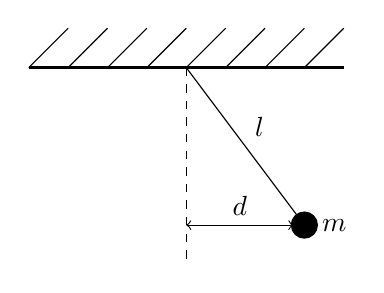
\begin{tikzpicture}
            \draw[thick] (-2,2) -- (2,2);
            \foreach \p in {-2,-1.5,...,1.5}
                \draw (\p,2) -- (\p+0.5,2.5);
            \draw[dashed] (0,2) -- (0,-0.5);
            \draw (0,2) -- (1.5,0) node[pos = 0.5, anchor = south west] {$l$} node[fill=black, draw=black, shape=circle] {} node[right] at (1.6,0) {$m$};
            \draw[<->] (0,0) -- (1.36,0) node[pos=0.5, above] {$d$};
        \end{tikzpicture}
    \end{center}
    Note that $ [p]=T, [m]=M, [g]=LT^{-2}, [l]=[d]=L $. Choose $m,g,l$ as independent quantities\footnote{$l$ is more suitable than $d$ since $l$ does not depend on initial displacement.}. Hence 
    \[
        p = f\left( \frac{d}{l} \right)m^{p_1}l^{p_2}g^{p_3} \Longrightarrow T=M^{p_1}L^{p_2+p_3}T^{-2p_3}.
    \]
    Balance dimensions gives $ p_1=0, p_2= 1/2, p_3=-1/2$, and thus 
    \[
        p = f\left( \frac{d}{l} \right) \sqrt{\frac{l}{g}}.
    \]
\end{example}
\begin{example}[Taylor's estimate of energy of the 1st atomic explosion]
    Let $ R(t) $ be the size of a fireball as a function of time. It has dimension $ L $. The density of air $\rho$ has dimensions $ ML^{-3} $ and the energy of explosion $E$ has dimensions $ ML^2T^{-2} $. We can write 
    \[
        R = C t^{\alpha}\rho^{\beta}E^{\gamma}\Longrightarrow L=L^{2\gamma-3\beta}M^{\beta+\gamma}T^{\alpha-2\gamma}.
    \]
    Hence $ \alpha=2/5 , \beta=-1/5,\gamma=1/5 $. Hence
    \[
        R(t)=C t^{2/5}\rho^{-1/5}E^{1/5} \Longrightarrow E = \frac{\rho R^5}{C^5 t^2}.
    \]
    Note that by measurement of the photographs of explosion,
    \[
        \frac{R^5}{t^2} \approx 6.7 \times 10^{13} \mathrm{m}^5 \mathrm{t}^{-2},\quad \rho \approx 1.25 \mathrm{kg} \mathrm{m}^{-3}.
    \]
    If $C\approx 1$ then $ E \approx 10^{14}J \approx 24 \times 10^{3} \text{ tonnes of TNT} $.
\end{example}